\documentclass[12pt,]{article}
\usepackage{lmodern}
\usepackage{setspace}
\setstretch{1.5}
\usepackage{amssymb,amsmath}
\usepackage{ifxetex,ifluatex}
\usepackage{fixltx2e} % provides \textsubscript
\ifnum 0\ifxetex 1\fi\ifluatex 1\fi=0 % if pdftex
  \usepackage[T1]{fontenc}
  \usepackage[utf8]{inputenc}
\else % if luatex or xelatex
  \ifxetex
    \usepackage{mathspec}
  \else
    \usepackage{fontspec}
  \fi
  \defaultfontfeatures{Ligatures=TeX,Scale=MatchLowercase}
    \setmainfont[]{Times New Roman}
\fi
% use upquote if available, for straight quotes in verbatim environments
\IfFileExists{upquote.sty}{\usepackage{upquote}}{}
% use microtype if available
\IfFileExists{microtype.sty}{%
\usepackage{microtype}
\UseMicrotypeSet[protrusion]{basicmath} % disable protrusion for tt fonts
}{}
\usepackage[left=1.2in,right=1.2in,top=1.5in,bottom=1.5in]{geometry}
\usepackage{hyperref}
\PassOptionsToPackage{usenames,dvipsnames}{color} % color is loaded by hyperref
\hypersetup{unicode=true,
            pdftitle={Vulnerable Growth: Comment},
            pdfauthor={Lluc Puig-Codina},
            colorlinks=true,
            linkcolor=Maroon,
            citecolor=Blue,
            urlcolor=blue,
            breaklinks=true}
\urlstyle{same}  % don't use monospace font for urls
\usepackage{graphicx,grffile}
\makeatletter
\def\maxwidth{\ifdim\Gin@nat@width>\linewidth\linewidth\else\Gin@nat@width\fi}
\def\maxheight{\ifdim\Gin@nat@height>\textheight\textheight\else\Gin@nat@height\fi}
\makeatother
% Scale images if necessary, so that they will not overflow the page
% margins by default, and it is still possible to overwrite the defaults
% using explicit options in \includegraphics[width, height, ...]{}
\setkeys{Gin}{width=\maxwidth,height=\maxheight,keepaspectratio}
\IfFileExists{parskip.sty}{%
\usepackage{parskip}
}{% else
\setlength{\parindent}{0pt}
\setlength{\parskip}{6pt plus 2pt minus 1pt}
}
\setlength{\emergencystretch}{3em}  % prevent overfull lines
\providecommand{\tightlist}{%
  \setlength{\itemsep}{0pt}\setlength{\parskip}{0pt}}
\setcounter{secnumdepth}{0}
% Redefines (sub)paragraphs to behave more like sections
\ifx\paragraph\undefined\else
\let\oldparagraph\paragraph
\renewcommand{\paragraph}[1]{\oldparagraph{#1}\mbox{}}
\fi
\ifx\subparagraph\undefined\else
\let\oldsubparagraph\subparagraph
\renewcommand{\subparagraph}[1]{\oldsubparagraph{#1}\mbox{}}
\fi

%%% Use protect on footnotes to avoid problems with footnotes in titles
\let\rmarkdownfootnote\footnote%
\def\footnote{\protect\rmarkdownfootnote}

%%% Change title format to be more compact
\usepackage{titling}

% Create subtitle command for use in maketitle
\providecommand{\subtitle}[1]{
  \posttitle{
    \begin{center}\large#1\end{center}
    }
}

\setlength{\droptitle}{-2em}

  \title{Vulnerable Growth: Comment}
    \pretitle{\vspace{\droptitle}\centering\huge}
  \posttitle{\par}
    \author{Lluc Puig-Codina\footnote{\href{mailto:llucpuigcodina@gmail.com}{\nolinkurl{llucpuigcodina@gmail.com}};
  The views expressed in this document reflect those of the author and
  are not necessarily shared by the European Central Bank. This research
  did not receive any funding from agencies in the public, commercial or
  not-for-profit sectors. I would like to thank Adrian Pagan for his
  helpful comments and suggestions. All errors are my own.}}
    \preauthor{\centering\large\emph}
  \postauthor{\par}
    \date{}
    \predate{}\postdate{}
  
\usepackage{booktabs}
\usepackage{longtable}
\usepackage{caption}
\captionsetup[figure]{labelformat=empty}

\begin{document}
\maketitle

\newpage

\abstract{\textit{Adrian et al. (2019) study the conditional distribution of GDP growth, finding a tight relationship between downside risks and financial conditions. Herein I examine the robustness of their conclusions. The main findings are: \textbf{i.} One-year-ahead predictive distributions show no evidence of conditional skewness, \textbf{ii.} Inference is based upon taking  some parameter estimates as true values or using wrong critical values, \textbf{iii.} Methodological shortcomings related to the fitting of the skewed t-Student distribution \textbf{iv.} Incorrect claims about model properties and its interpretation are made.} (JEL C53, E27, E32, E44)}

\vspace{0.5cm}

Adrian et al.~(2019) - henceforth ABG - argue that there is a connection
between future real GDP growth and deteriorating financial conditions
today. The first piece of evidence put forward to motivate such
connection is a three dimensional plot of a remarkable aesthetic, ABG
Figure 1, showing the one-year-ahead predicted conditional distribution
of real GDP growth across time. The figure is used to summarize and
present several of their main findings, ABG page 1264:

\begin{quote}
Two features are striking about the estimated distribution. First, the
entire distribution, and not just the central tendency, evolves over
time. For example, recessions are associated with left-skewed
distributions while, during expansions, the conditional distribution is
closer to being symmetric. Second, the probability distributions inherit
the stability of the right tail from the estimated quantile
distribution, while the median and the left tail of the distribution
exhibit strong time series variation. This asymmetry in the evolution of
the conditional distribution of future GDP growth indicates that
downside risk to growth varies much more strongly over time than upside
risk.
\end{quote}

This article asks how robust their conclusions are to various issues
that arise with the methods they employ.

\hypertarget{i.-the-mechanism-quantile-regressions}{%
\section{I. The Mechanism: Quantile
Regressions}\label{i.-the-mechanism-quantile-regressions}}

The first step in documenting a relationship between financial
conditions, measured by the National Financial Conditions Index (NFCI),
and real GDP growth is presented in the univariate quantile regressions
of ABG Figure 3. The dependent variable is either one-year-ahead or
one-quarter ahead real GDP growth. The independent variable is either
current NFCI or current real GDP growth. The authors show that quantile
regression slopes are similar at different percentiles for current real
GDP growth, but regression slopes present large changes across
percentiles for NFCI, implying an asymmetric response of future real GDP
growth to financial conditions. In particular, slopes are close to 0 for
the 95 percentile, while for the 5 percentile they are steep and
negative. Despite the authors reassurance that ``regression slopes for
the NFCI do not change significantly when current GDP growth is also
included in the regression'', they do. For the one-year-ahead
specification, the 95 percent quantile regression slope of NFCI goes
from 0.2247191 to 1.3776231 when current real GDP growth is included.
This can be clearly seen by comparing results in ABG Figure 3 Panel D
with Figure 4 Panel D. Despite being an extreme percentile, the fitted
values from this regression will be key in the construction of the
conditional distributions shown in ABG Figure 1 and Figure 5 Panel B.

Then, ABG move on present further evidence interpreted as indicative of
a non-linear relationship between real GDP growth and financial
conditions, ABG page 1269:

\begin{quote}
Figure 4 shows that, at both the lower and the upper quantiles, the
estimated slopes are significantly different at the 10 percent level,
from the OLS slope.\textsuperscript{5}
\end{quote}

To get their Figure 4 involves two steps. First, multivariate quantile
regressions were estimated at percentile
\(\tau \in \{0.05, 0.1,\dots, 0.95\}\) using the actual data. The second
step involved estimating a bivariate VAR(4) and simulating 1000 samples
using normal innovations. For each of the simulated samples a quantile
regression at \(\tau\) is fitted and the median of the slopes found,
along with 68, 90 and 95 percent confidence intervals (CIs). If the
point estimates using the actual data are outside the CIs of the
estimated slopes using simulated data, ABG conclude that the regression
slopes are different. Under the authors interpretation of the results,
the relevant null hypothesis is
\(\widehat{\beta(\tau)^{sim}} - \widehat{\beta(\tau)^{orig}} = 0\).\footnote{Say only for a particular variable and percentile, thus sidestepping the issue of multiple hypothesis testing.}
Yet the procedure seems to ignore the uncertainty in the estimation of
the regression slope on the original data, whose CIs are never reported,
treating it as a constant. Therefore, the test holds valid only if we
assume the point estimate of the regression slope to be the true
parameter, an unreliable assumption for proper inference.

As an additional note of caution, notice that in all specifications GDP
enters the quantile regression and VAR in growth rates, while NFCI
enters the regression and VAR in levels. Such setting implies that if
the relationship is to be interpreted as causal, financial shocks have a
permanent effect on upon the \textit{level of GDP}.

\hypertarget{ii.-predictive-distributions-and-skewed-t-student-fitting}{%
\section{II. Predictive Distributions and Skewed t-Student
Fitting}\label{ii.-predictive-distributions-and-skewed-t-student-fitting}}

As described in the paper, ABG Figure 5 reports the fitted values of
quantile regression at the 5, 25, 50, 75 and 95 percentiles, alongside
the realization of real GDP growth. ABG Figure 5 Panel B can be
interpreted as a `raw' version of Figure 1 in
ABG\footnote{If we only use the 5, 25, 75 and 95 percentiles.}, before
fitting the skewed t-Student. Therefore, many of the properties found in
Figure 1 of ABG should also be found in ABG Figure 5 Panel B. If we want
to focus on time varying skewness, both figures are difficult to
interpret. Many things happen at the same time: location shifts, changes
in the variance, skewness and so on. In order to better appreciate time
varying skewness in the predictive distributions one could center Figure
5 Panel B of ABG around the conditional mean. This is what I present in
Figure 1. The conditional mean is estimated via OLS regression:
\(\widehat{\mathbf{E}\{y_{t+h} | x_t \}} = \widehat{\beta_0^{OLS}} + \widehat{\beta_1^{OLS}}x_t\);
where \(y_{t+h}\) is annualized average real GDP growth between \(t+1\)
and \(t+h\), and \(x_t\) is a vector containing current real GDP growth
and NFCI.

\[
\text{[Figure 1 here]}
\]

At glance at the figure shows that, after removing changes in the mean,
the One-Year-ahead specification exhibits neither asymmetry nor time
varying skewness. At the very least one can certainly see that the
distribution does not exhibit greater left skewness during recessions as
ABG claim.

Another piece of evidence on the lack of such skewness during recessions
is presented in ABG Figure A.2. (b), which plots the evolution of the
estimated skewed t-Student shape parameter for the One-Year-Ahead
specification. There seems to be either none or very little relationship
between the shape parameter and recessions. Even though the authors note
this, and point to changes in the location and scale parameters as the
main drivers of the conditional distribution, it hasn't prevented them
from citing skewness as evident in ABG Figure 1.

A closer examination of ABG's method is warranted. After obtaining the
fitted values from quantile regression at the 5, 25, 75 and 95
percentiles, a skewed t-Student is selected and its four parameters are
chosen to minimize, at every \(t\), the sum of square distances between
the regression estimated quantiles and the distribution implied
quantiles. In the matching, bounds are imposed on the values of the
parameters.\footnote{$-20 \leq \mu \leq 20$; $0 < \sigma \leq 50$; $-30 \leq \alpha \leq 30$; and $\nu \in \{1,2, \dots,30\}$. Due to the degrees of freedom being discrete, AGBs optimization consists of grid search over a restricted parameter space for the degrees of freedom, bringing into question claims about computational efficiency.}
The attractive use of the skewed t-Student in this application is that
the conditional mean, variance, skewness and kurtosis of the stochastic
process can be time varying. Moreover, subject to some regularity
constraints, the estimation is exactly identified. An issue that is
naturally raised here is that one could choose a different quadruple of
percentiles and these could possibly give different parameter estimates.
ABG are silent as to why they choose the quadruple of (5, 25, 75 and
95)th percentiles. Without knowing how large is the uncertainty around
those estimates, as in prediction intervals, which could be high for
extreme quantiles such as the 5 and 95 percentiles, one is also unable
to know how accurate are the distributions presented in Figure 1 of ABG.

The estimated parameters are reported in ABG Figures A.1 and A.2, which
I believe are important figures to understand the results of their
method. As an illustration I reproduce ABG Figure A.1 and A.2 in Figure
2 and 3 using not only their selected percentiles (blue) but also an
alternative skewed \(t\)-distribution parameter estimation using the
quadruple of (20, 40, 60 and 80)th percentiles (red). It is clear that
there are large differences between the estimated parameters from the
use of different percentiles. Such large differences in the parameters
will also translate in large differences for estimated risk measures
such as Expected
Shortfall.\footnote{Another issue to be raised is that of quantile crossing, which violates the monotonicity condition of the quantile function. Quantile crossing can be observed in ABG Figure 7 at many panels, where the raw CDF decreases. Some of this issues are not new, Fan and Fan (2006) show that quantile autoregression produces inconsistent estimates and is highly sensible to misspecification when conditional quantiles are not strictly increasing in $\tau$.}

\[
\text{[Figure 2 here]}
\]

\[
\text{[Figure 3 here]}
\]

\hypertarget{iii.-alternative-approaches-and-out-of-sample-evidence}{%
\section{III. Alternative Approaches and Out of Sample
Evidence}\label{iii.-alternative-approaches-and-out-of-sample-evidence}}

ABG employ two other econometric models which they claim result in
findings similar to what is obtained using their main methodology. It is
implied that such exercises provide robustness to their conclusions. The
first approach was to fit a conditionally heteroskedastic model of the
form:

\begin{align}
y_{t+1} = \gamma_0 + \gamma_1 x_t + \sigma_t\varepsilon_{t+1}; \ \ \ \ \ln(\sigma^2_t) = \delta_0 + \delta_1 x_t
\end{align}

where \(y_{t+1}\) is real GDP growth next quarter and \(x_t\) a vector
with current NFCI and real GDP growth. The error term is assumed to be
normally distributed, \(\varepsilon_{t+1} \sim \mathcal{N}(0,1)\).
Therefore, the conditional distribution is:

\begin{align}
y_{t+1}|x_t \sim \mathcal{N}(\gamma_0 + \gamma_1 x_t, e^{\delta_0 + \delta_1 x_t})
\end{align}

i.e.~it is normal, and so there is no skewness in it. It is therefore
difficult to conclude that there is (ABG page 1281):

\begin{quote}
The simple conditionally heteroskedastic model is able to reproduce the
strongly skewed conditional GDP distribution by simply shifting the mean
and volatility of GDP as a function of economic and financial
conditions.
\end{quote}

Finally, we can turn to the out-of-sample evidence. In order to
back-test the model ABG use the test developed in Rossi and Sekhposyan
(2019), whose results are shown in ABG Figure 11 Panel C and D. The test
is based on the fact that a random variable evaluated at its own CDF
follows a standard uniform distribution. This is known as the
probability integral transforms (PITs) and involves using one step ahead
CDFs of the estimated t-Students evaluated at their realization. The
closer the CDF of the PITs is to the 45 degree line the better.

The authors interpret the results in the following way (ABG page 1279):

\begin{quote}
For both the full conditional predictive distribution and the predictive
distribution that conditions on economic conditions only, the empirical
distribution of the PITs is well within the confidence bands for the
lower quantiles, though the empirical distribution falls outside the
confidence band in the center of the distribution.
\end{quote}

This interpretation is incorrect. The confidence bounds used in ABG
correspond to the null hypothesis of the
\textit{full distribution being correctly specified}.\footnote{In the replication codes \texttt{VulnerabilityOutOfSample.m} line 333-4 the critical value is defined for the One-Quarter-Ahead Specification, $\kappa$ = 1.34. In Rossi and Sekhposyan (2019) Table 1 Panel A, 1.34 is the critical value corresponding to a test on the whole distribution.}
Therefore, the correct interpretation is that at one quarter ahead we
can reject the null of the full distribution being correctly specified
for both the ``only GDP'' and ``GDP and NFCI''. In the case of
one-year-ahead, we can't reject the null for both models. Nothing can be
said about other percentile ranges with those CIs. A remarkable fact
from ABG Figure 11 Panel C and D is that the model with GDP only seems
to almost always be closer to the 45 degree line than the model with GDP
and NFCI. In addition, there seems to be some discrepancies between the
test as described in Rossi and Sekhposyan (2019) and the implementation
in ABG, see the Appendix.

If instead of testing the null of the full distribution being correctly
specified we only want to test that the left tail, say
\(\tau \in [0, 0.25]\), is correctly specified, as ABG seem to intend,
the corresponding critical value is a smaller one, yielding smaller
CIs.\footnote{$\kappa = 1$  as reported in Table 1 Panel B of Rossi and Sekhposyan (2019) for one step ahead forecasts.}
For this exercise, instead of using an expanding window, as ABG do, I
use a moving window, as is appropriate for the test. Therefore, I use
data from 1973:I to 1992:IV to estimate the predictive distribution for
1993:I (one quarter ahead) and 1993:IV (one year
ahead).\footnote{Despite ABG describing their exercise in a similar manner their first predictive density out of sample is for 1993:II (one quarter ahead) and 1994:I (one year ahead). One can easily observe this by noting that from and including 1993:I to 2015:IV there are 92 quarters, but the object \texttt{PitST\_OOS} in code \texttt{VulnerabilityOutOfSample.m} only contains 91 values.}
Then I use data from 1973:II to 1993:I to estimate the predictive
distribution for 1993:II (one quarter ahead) and 1994:I (one year
ahead), and so on until a 2015:IV forecast. Results are shown in Table
1. If the statistic is larger than the critical value we can reject the
null hypothesis of the conditional left tail being correctly
specified.\footnote{For the One-Year-Ahead specifications I have followed ABG in implementing the multi-step ahead version of the test, although the forecast seems to be direct. If I was to use the critical values of the one-step test, 1 and 0.34, the conclusions remain unaltered.}
Both at One-Quarter and One-Year-Ahead we can reject the null of the
left tail being correctly specified for ``NFCI and GDP'', but not for
``only GDP''.

\[
\text{[Table 1 here]}
\]

\hypertarget{iv.-discussion}{%
\section{IV. Discussion}\label{iv.-discussion}}

There seem to be shortcomings in the analysis which raise concerns about
the overall robustness of the results and the reliability of the method.
The same method has been used in Chapter 2 of the IMF Global Financial
Conditions Report since October 2017 and is the same one underpinning
the IMF Growth-at-Risk
tool\footnote{IMF. 2019. “Growth-at-Risk Tool” \textit{Github}, Februrary 22. \url{https://github.com/IMFGAR/GaR}. Aside from the issues raised in this comment, in the technical documentation one can find some disturbing remarks regarding implementation: “To avoid that the t-skew parametrization converges towards a Gaussian (infinite degrees of freedom), the tool anchors the degrees of freedom at 2.”},
which has been used in several article IV country reports. The method
has also been extended to study the term structure of growth at risk,
Adrian et. al.~(2018) and house prices at risk, IMF Global Financial
Stability report April 2019.

\hypertarget{references}{%
\section{References}\label{references}}

\textbf{Adrian, Tobias, Nina Boyarchenko, and Domenico Giannone}. 2019.
``Vulnerable Growth.'' \emph{American Economic Review} 109 (4): 1263-89.

\textbf{Adrian, Tobias, Grinberg, Federico, Liang, Nellie, and Malik,
Sheheryar.} 2018. ``The term structure of growth-at-risk.''
International Monetary Fund.

\textbf{Fan, Jianqing, and Yingying Fan.} 2010. ``Issues on quantile
autoregression.'' Unpublished.

\textbf{Rossi, Barbara, and Sekhposyan, Tatevik.} 2019. ``Alternative
tests for correct specification of conditional predictive densities.''
\emph{Journal of Econometrics} 208 (2): 638-657.

\hypertarget{tables}{%
\section{Tables}\label{tables}}

\begin{longtable}{lrrrr}
\caption{\label{tab:table1}Correct Specification Tests of the Conditional Left Tail}\\
\toprule
\multicolumn{1}{c}{ } & \multicolumn{2}{c}{Kolmogorov-Smirnov Test} & \multicolumn{2}{c}{Cràmer-von Mises Test} \\
\cmidrule(l{3pt}r{3pt}){2-3} \cmidrule(l{3pt}r{3pt}){4-5}
  & Statistic & Critical Value at 95\% & Statistic & Critical Value at 95\%\\
\midrule
One-Quarter-Ahead GDP and NFCI & 1.45 & 1.00 & 1.02 & 0.34\\
One-Quarter-Ahead only GDP & 0.49 & 1.00 & 0.05 & 0.34\\
One-Year-Ahead GDP and NFCI & 2.39 & 1.92 & 2.48 & 1.98\\
One-Year-Ahead only GDP & 0.52 & 1.63 & 0.05 & 0.99\\
\bottomrule
\end{longtable}

\hypertarget{figures}{%
\section{Figures}\label{figures}}

\begin{figure}
\centering
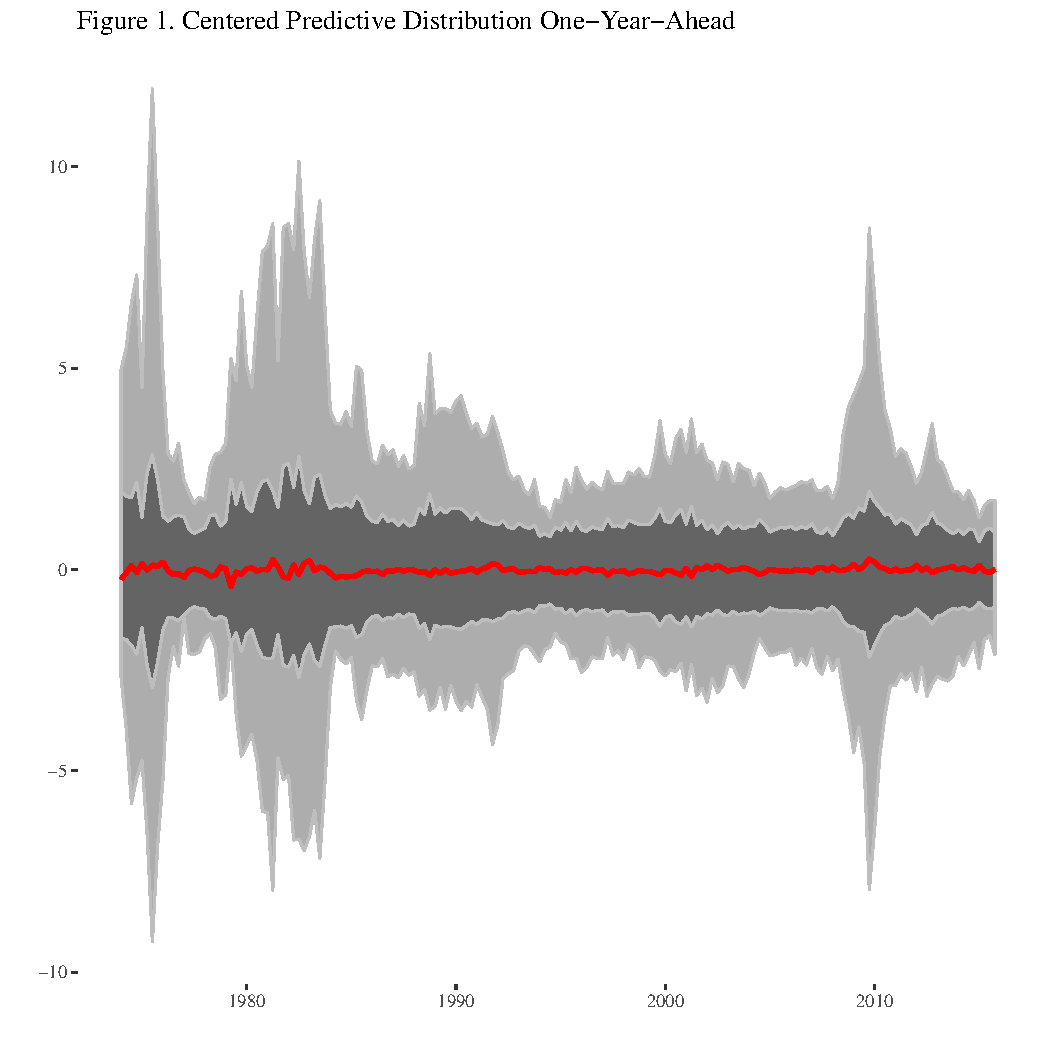
\includegraphics{figures/figure1.pdf}
\caption{\emph{Note}: The figure shows the time series evolution of the
centered predicted distributions of one-year-ahead real GDP growth.}
\end{figure}

\begin{figure}
\centering
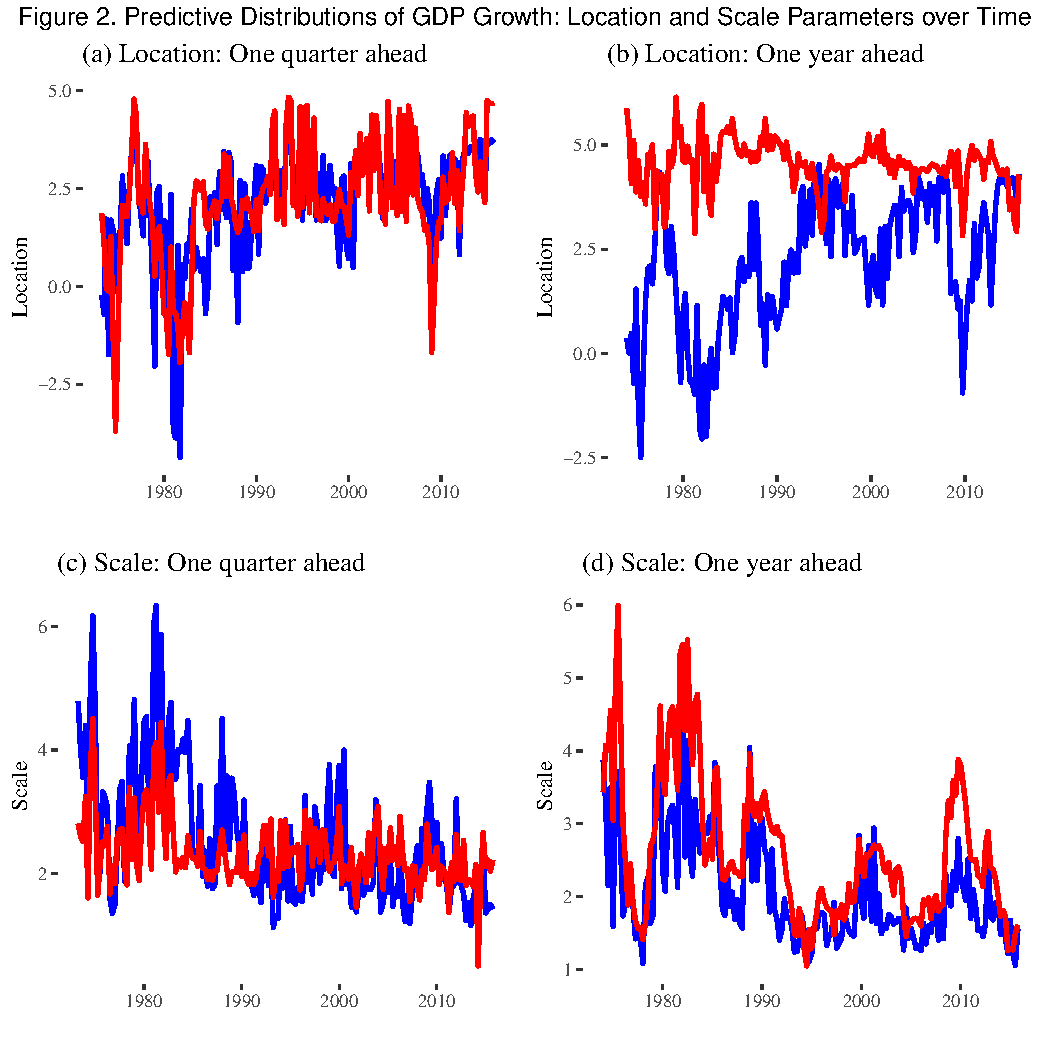
\includegraphics{figures/figure2.pdf}
\caption{\emph{Note}: The figure shows the time series evolution of
location \(\mu_t\) and scale \(\sigma_t\). The blue line shows the
specification using the 5, 25, 75 and 95 percentiles while the red line
shows the specification using the 20, 40, 60 and 80 percentiles.}
\end{figure}

\begin{figure}
\centering
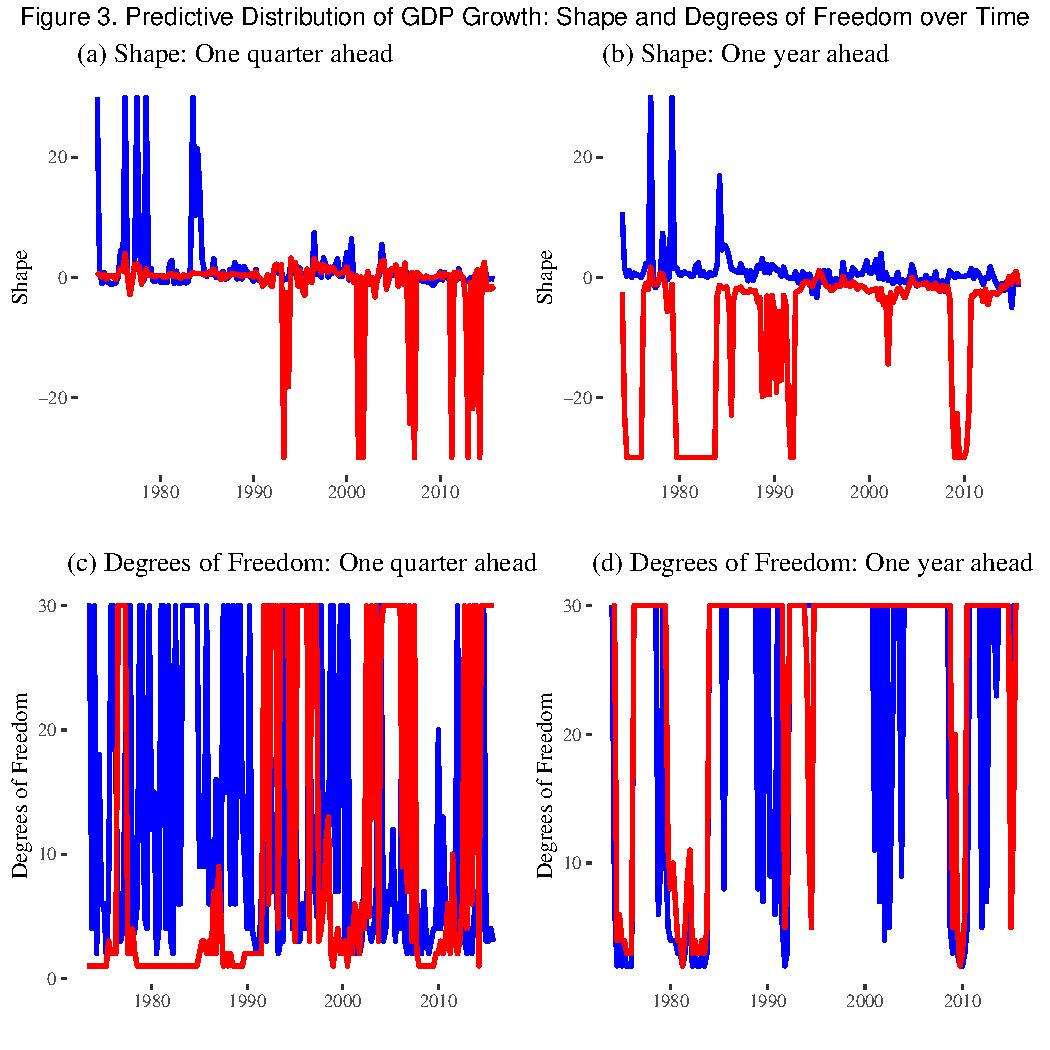
\includegraphics{figures/figure3.pdf}
\caption{\emph{Note}: The figure shows the time series evolution of
location shape \(\alpha_t\) and degrees of freedom \(\nu_t\). The blue
line shows the specification using the 5, 25, 75 and 95 percentiles
while the red line shows the specification using the 20, 40, 60 and 80
percentiles.}
\end{figure}

\newpage

\hypertarget{appendix}{%
\section{Appendix}\label{appendix}}

\hypertarget{implementation-of-rossi-and-sekhposyan-2019}{%
\subsection{Implementation of Rossi and Sekhposyan
(2019)}\label{implementation-of-rossi-and-sekhposyan-2019}}

Right after stating Assumption 3, Rossi and Sekhposyan (2019) define the
bootstrap statistic as:

\[
\Psi_P^*(r; \omega) = P^{-1/2}\sum_{j=R}^{T-l+1}\eta_j \sum_{i=j}^{j+l-1} \left ( 1\{z_{i+h}(\omega) \leq r \} - \frac{1}{P}\sum_{t=R}^{T}1\{z_{t+h}(\omega) \leq r \} \right )
\]

The replication code \texttt{CVfinalbootstrapInoue.m} of ABG, instead of
implementing the above estimator, seems to implement the following as
the boostrap statistic:

\[
\Psi_P^*(r; \omega) = P^{-1/2}\sum_{j=R}^{T-l+1}\eta_j \sum_{i=j}^{j+l-1} \left ( 1\{z_{i+h}(\omega) \leq r \} - r \right )
\]

This difference can be clearly observed if one compares the
implementation of ABG with the implementation found in
\href{http://www.tateviksekhposyan.org/example.zip}{Sekhposyan's
website}.


\end{document}
